\chapter{Theoretical Background}
\label{theoretical_background}
This chapter covers the needed theoretical background about the topics discussed in this thesis.

\section{ROS}
ROS (Robot Operating System) is an open source project developed by the ``Open Source Robotics Foundation''. Like the name suggests it is an entire operating system for robots including hardware abstraction, low-level device control, implementation of commonly used functionality, communication between processes and package management.\\
Furthermore it provides tools and libraries to write, build and run code across multiple computers\cite{rosintro}.\\

\subsection{Packages}
This is the main structure for software in ROS. A package can contain many different nodes, libraries, service etc.. Furthermore it is the smallest possible structure that can be build by ROS\cite{rosconcepts}.
\subsection{Nodes}
Nodes are processes that perform computation. Since ROS is very fine granular, a system, that controls an entire robot can contain many nodes that are connected using topics. A package can be written with the use of one of the client libraries roscpp or rospy\cite{rosconcepts}.
\subsection{Plugins}

Plugins are a software type introduced by the pluginlib package that is a component of ``ros\_core''. Plugins are classes, that comply with a certain plugin interface. This allows to change the behavior of a node by loading different plugins for a certain task. Like this the original source code of the node does not need to be modified\cite{pluginlib}.

\subsection{Topics and Services}
All of the ROS nodes are connected with a publisher/subscriber like structure. The topic is basically just a name for a certain message.\\

Not only one node but unlimited many nodes can publish and subscribe to one topic. This generally can be seen like a message bus with not limited connection permissions\cite{rosconcepts}.

Unfortunately, the topic system is not well fitted for request and answers between two nodes, therefore the service structure has been implemented.\\ 
A node might offer a service under a certain node and another node can call that service. Services can have any in- and output that can be specified in a ``.srv'' file\cite{rosconcepts}.

\subsection{rviz}
rviz is a 3D visualization tool offered by default in ROS. It offers functionality to visualize sensor and further geometric data.\\
\subsection{rqt}
rqt is a qt based tool for the development of GUI's for the ROS framework\cite{rqt}.
\subsubsection{rqt\_reconfigure}
	rqt\_reconfigure is a plugin, for rqt, that provides functionality to edit parameters of the running nodes during runtime using an intuitive GUI\cite{rqtrecon}.
	
\subsubsection{rqt\_graph}

	rqt\_graph is a plugin for rqt, that offers a GUI, that displays the ROS computation graph and therfore all active nodes and their connection via topics\cite{rqtgraph}.
\subsubsection{rqt\_tf\_tree}
	rqt\_tf\_tree can be used to display the tf\_tree of the current system. It displays all tf frames and their hierarchic structure\cite{rqttftree}.
\subsection{REP}
REP's (short for ROS enhanced proposals) are guidelines made and maintained by the ROS community. It is highly advisable to follow the guidelines as much as possible.

Complying to these guidelines allows external people easier comprehension of the structure of the robot and eliminates misunderstandings.

The most important REP's in this project are REP 103 and REP 105.
\subsubsection{REP 103}
	
	"This REP provides a reference for the units and coordinate conventions used within ROS"\cite{REP103}\\  
	
	\textbf{Coordinate Frame}
	\begin{itemize}
		\item \textbf{X-Axis} - forward
		\item \textbf{Y-Axis} - left
		\item \textbf{Z-Axis} - up
	\end{itemize}
	
	\textbf{Units}\\
	
	Units will always be represented in SI units and their derived units.\\
	
	\textbf{The order of preference for rotations}
	\begin{enumerate}
		\item Quaternion
		\item Rotation matrix
		\item Fixed axis roll, pitch, yaw
		\item Euler angles
	\end{enumerate}
	\cite{REP103}
	
\subsubsection{REP 105}
	"This REP specifies naming conventions and semantic meaning for coordinate frames of mobile platforms used with ROS."\cite{REP105}\\
	
	REP103 Applies for all fixed coordinate frames.
	
	\textbf{Coordinate Frames}
	\begin{itemize}
		\item \textbf{base\_link} is a fixed frame on the robot base. It serves as the reference points for all of hardware mounted on the robot itself like sensors.
		\item \textbf{odom} is a world fixed frame that serves as the reference for the pose of the robot.\\ Since the pose of the robot will drift over time, it wont serve as a good long term reference.\\In most cases the odom frame will be computed using localization sensors like wheel odometry, imu's, visual odometry, etc. which leads to a continuous frame.
		\item \textbf{map} is a world fixed coordinate frame that serves as the reference for the odometry frame. It is also the base for a map of the environment such as the ones provided by slam algorithms. The frame is time discrete since it is mostly computed by localization algorithms.
	\end{itemize}
	
	That tree can be extended by an earth frame that would be the reference for the localization of the map in the earth. Which is useful, for long range robot platforms.\cite{REP105}
	
	
	
\subsection{tf}
In most cases robots that are controlled by ROS have a tf\_tree. This tree is the coordinate frame structure of the robot. This tf\_tree includes a coordinate frame for every sensor and actor.\\
 The structure in most trees of mobile platforms is quite similar which is due to the REP105 (ROS enhanced proposals). This contains a definition of recommended names for the robot frames and their order in the tf tree. But it should be noted that not every frame that is defined in the norm has to be in every tree. The basic structure starts with a fixed frame. This frame will be the not changing frame in the environment. For moving robots this is often earth, map or odom, while in stationary robots this can even be base\_link.\\
 

The tree is normally build up like in Figure \ref{stdtftree}.


\begin{figure}[H]
	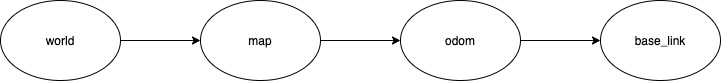
\includegraphics[width=\textwidth]{Pictures/tf standard tree}
	\caption{standard tf tree}
	\label{stdtftree}
\end{figure}

TF2 is the successor of TF and is a very powerful tool in the ROS environment. With this it is possible to transform sensor\_msgs and geometry\_msgs from one frame in another. Furthermore it offers the possibility to transform old data into the present or at any other point in the past.

\subsection{URDF and Xacro}
The robot hardware description consists of one or more URDF(Unified Robot Description Format) based XML files. Their purpose is to define the geometric shape of every part of the robot. 

\subsection{robot\_state\_publisher}
	This package uses the robot hardware description and builds up the tf\_tree using static\_transform\_publishers.


\subsection{move\_base}
Move\_base is an implementation of an action, that tries to control a mobile platform to get as close to a given goal as possible. It offers an implementation of the costmap\_2d package and supports any global and local planner, that adheres to the interface defined by the nav\_core package\cite{movebase}.

\subsection{nav\_core}
This package include common interfaces for the global and local planners used in move\_base.

Furthermore it provides an interface for recovery behaviours\cite{navcore}.

\subsection{Global Planner}
The global planner in move\_base has the task of finding a path from start to goal in the global costmap, without going through lethal cells. The shape of the robot is not directly considered by the global planner for collision checking. Only the collision with lethal cells of the costmap is respected.

\subsubsection{base\_global\_planner}
This is the default global planner of move\_base. It features Dijkstra and A* path finding algorithms.\\

Dijkstra does only consider determines the cost to get from the start node to every other node, until it finds the goal. From this goal Dijkstra can backtrack the shortest/cheapest path.\cite{AlgorithmenundDatenstrukturen}.\\

A* is based on the Dijkstra algorithm but has one main difference. It considers not only the cost from the start to the current cell in the grid, but as well a heuristic parameter, which is a general guess for the cost from the cell to the goal. The heuristic parameter is mostly bound to the euclidean distance between the cell in the grid and the goal cell. Like this the parameter will never overestimate the actual cost of the path\cite{AlgorithmenundDatenstrukturen}. This weights cells that are in the general direction to the goal more then other cells and in certain situations speeds up the path finding.\\

\subsection{Local Planner}
The local planner is meant to produce a feasible path, that generally follows the path produced by the global planner. It takes care of collision avoidance and considers the dynamic of the robot itself.

\subsubsection{teb\_local\_planner}
teb\_local\_planner is a plugin for move\_base. In contrast to other local planners it uses a so called timed elastic band algorithm. This is an extension to the elastic band approach which does not take any dynamic constraints of the robot into account.\cite{Rsmann2012TrajectoryMC}.

The elastic band approach can be described as a series of nodes that are interconnected with springs, that try to pull the nodes into a straight line, which is often described as the internal force. The external force is a repelling force caused by obstacles on the path\cite{elasticband}.

\subsubsection{dwa\_local\_planner}
dwa\_local\_planner uses as the name suggests a dynamic window approach. This approach is based on a dynamic window defined by the maximum values for the robots acceleration velocity in all of the dimensions relevant for 2D operation.\\
The algorithm generates a set of possible trajectories based on the dynamic constraints, a given time frame, the local costmap and the global plan and selects the ``best'' trajectory\cite{dwa}.

Since the planner only considers a set of trajectories, that are not influenced by the environment, tuning of the planner is difficult. 
This can be justified, by the fact that a small variety of angular velocities would allow the planner to navigate in tight corridors, whereas it would hinder the turning capabilities in corners at the same translational speed.

\subsection{Costmap}
A costmap is a grid stile map and its purpose is to store information about obstacles in the surrounding of the robot.\\
There are two different costmaps, the global costmap and the local costmap.
The global costmap is by the global planner to find a collision free path, whereas the local costmap is used by the local planner for local planning.\cite{navsetup}\\

\begin{figure}[H]
\centering
	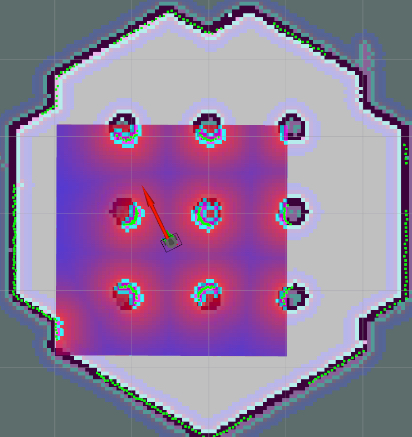
\includegraphics[width=.5\textwidth]{Pictures/inflationref}
	\caption{costmap with obstacles and inflation \cite{infl}}
	\label{costmap}
\end{figure}


\subsubsection{Cost values}
The values in a costmap can be in the range [0-255], but the underlying structure categorizes them in the following 3 sections:
\begin{itemize}
	\item Lethal obstacle - 254
	\item Free space - 0
	\item No information - 255
\end{itemize}

\subsection{Marking and Clearing}
Obstacles in the costmap can not only be marked, but also cleared by the subscribed data source. For each data source a configuration regarding the clearing and marking permissions is necessary.\\
For clearing the costmap uses a raytracing algorithm, which allows the costmap to handle moving obstacles\cite{costmap}. Raytracing is a rendering technique, that follows the trace of a ray, in order to determine the influence of that ray with objects. 
In this application, this is done by casting rays from the robot to the current measurement of the sensors, which allows to determine if a lethal cell in the costmap is feasible.
\subsubsection{Inflation}
Inflation is a process where a occupied cell is inflated by over the distance decreasing cost values for a configurable radius, as pictured in Figure \ref{costmap}.\\
This process is used by the default plugin inflation\_layer with the cost distribution pictured in Figure \ref{costdistribution}\cite{costmap}.

\begin{figure}[H]
	\centering
	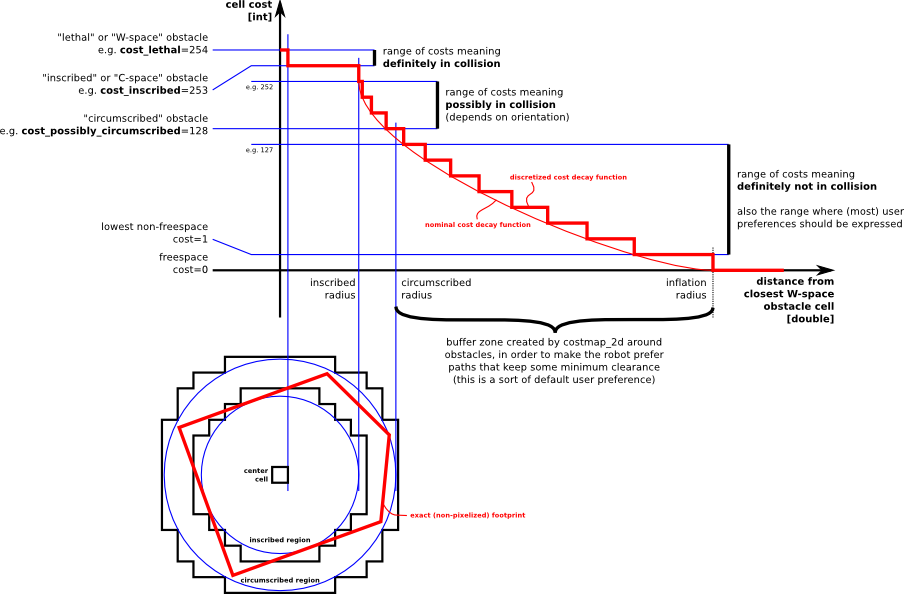
\includegraphics[width=\linewidth]{Pictures/costmapinflation}
	\caption{cost distribution and classification \cite{costmap}}
	\label{costdistribution}
\end{figure}

The usage of inflation has two reasons. First it is used to close gaps between two measured obstacles and therefore usefull, if the sensor resolution is relatively corse.\\
The second reason is to prevent the global planner from getting too close to obstacles, since it does not feature any collision checking, that considers the robot shape, but only checks for lethal cells in the costmap. Therefore the inflation radius is typically set to slightly more than the radius of the robot\cite{costmap}.

\subsubsection{Layer}
The costmap uses a layer structure of plugins that can handle different tasks. It finally combines the data from each layer, to produce the final costmap.\\

By default the costmap\_2d package offers the following 3 layers:
\begin{itemize}
	\item \textbf{Static map layer} is a layer that converts a prerecorded map into obstacles.
	\item  \textbf{Obstacle layer} is a plugin that handles input from sensor sources. The plugin marks and raytraces obstacles in 2D. It can handle LaserScans PointCloud and PointCloud2.
	\item \textbf{Inflation layer} handles the inflation of lethal obstacles in the costmap.
\end{itemize}

Furthermore the plugins Social ``Costmap Layer'' and ``Range Sensor Layer'' are offered.

Using the pluginlib interface and the costmap libraries custom layers for the costmap can be developed to achieve special behavior of the robot.

\section{SLAM}

SLAM (simultaneous localization and mapping) is a problem, where a map of the environment has to be build based on sensor data. During this the observer has to be continuously localized within the map.

\section{Google Cartographer}
Google Cartographer is a lidar based SLAM algorithm developed by Google. In contrast to gmapping it is based on loop closure to ensure real time mapping even in relatively big environments.\\
Submaps are considered for loop closure, if they are close to each other. A scan matcher tries to find constraints between the submaps and the current scan. When searching for loop closure constraints at a certain rate one can achieve basically instantaneous optimization of the map, just by the fact that the current scan is similar to one of the underlying submaps\cite{cartographer}.\\

\section{Edge Effect}

The edge effect is an error source during laser based distance measurement.
When the laser beam used for measurement is directly at an edge of an obstacle, this splits the beam or rather blocks a part of it. The resulting measurement lies in the range of all distances measured by the beam and is therefore located behind the real edge of the obstacle like further described in the paper of Klapa about the ``Edge effect and its impact upon the accuracy of 2D and 3D modeling using laser scanning'' \cite{edgeeffect}.\\


\section{Carolo-Cup}
The Carolo-Cup is an event hosted by Braunschweig University and is an event in which the teams of many different universities can compete against each other and present their work and progress in the field of autonomous driving.

The Cup offers a fair ground by reducing environmental influence like lighting but creates scenarios based on a realistic environment for the navigation. Judges from science and finance related fields will rate the individual teams based on static and dynamic events.

Static events are the concept, technical approaches, project management, presentation and the agenda of the teams, whereas the dynamic events are different for the two different difficulty levels.

The Basic-Cup covers free driving with and without static obstacles, as well as parking. The Master-Cup adds more difficulty by offering dynamic obstacles, traffic signs and variations of the road markings for no pass or express zones\cite{carolocup} \cite{vdecarolo}.

Robot restrictions relevant in this thesis:
\begin{itemize}
	\item \textbf{Scale} 1:10
	\item \textbf{Width} - max. 300mm
	\item \textbf{Wheel base} - min. 200mm
	\item \textbf{Steering} - at least one axle must be steerable
\end{itemize}

Track restrictions relevant in this thesis:
\begin{itemize}
	\item \textbf{lane width} 350-450mm
	\item \textbf{sharpest turn radius} 1000mm
\end{itemize}











\chapter{Requirements}
\label{requirements}

This chapter defines requirements for parts of this work, based on the scope of the thesis and the theoretical background.

\section{Robot and Environment}

The regulations of the Carolo-Cup strongly restrict the size and the steering type of the used robot. In this thesis these restrictions will be ignored, in order to use the mobile robotic platform Arlo from the manufacturer Parallax pictured in Figure \ref{arlore}. This platform is the default platform of the laboratory for mobile robotics at Aalen University\\

This decision is based on a potential comparisons after this thesis between real and simulated environments. This could give insight on problems in the navigation that have not yet been addressed.\\


\begin{figure}[H]
	\centering
	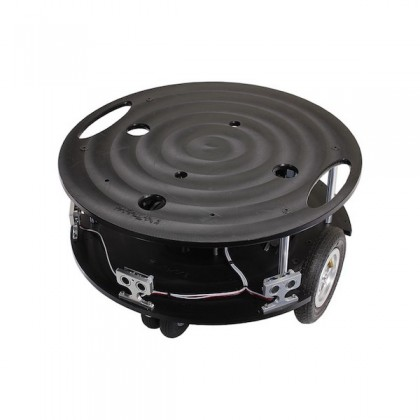
\includegraphics[width=.7\textwidth]{arlo real}
	
	\caption{mobile robot ``Parallax Arlo'' \cite{arloreal}}
	\label{arlore}
\end{figure}

As a consequence to the previous choice regarding the robot, the road has to be altered, so the proportions between robot size and road dimensions remain the same. Since the Arlo robot has a diameter of 450mm the track width is set to 900mm to keep the 1:2 scale. This 1:2 proportion can be deduced from the defined vehicle and road widths of the Carolo-Cup\cite{carolocup}.

The sensor setup of the robot is based on the anticipated tasks in the Carolo-Cup. 

Therefore the robot is equipped with the following sensors:

\begin{itemize}
	\item Lidar - obstacle detection
	\item Wheel encoders - odometry
	\item Camera - road detection
\end{itemize}

As the navigation might require additional input this is not a fixed requirement, but the initial configuration.

To keep the navigation software flexible, its output is defined as a vector of linear and angular velocity. This output is applicable for any type of steering.

\section{Software}
As mentioned in the introduction the navigation is developed for ROS-Noetic, furthermore roscpp (C++ library) is prefered over rospy (Python library) to keep the source code of developed ROS nodes as uniform as possible.

\section{Simulation}
Since the environment is simulated the simulator has to have the following features.
\begin{itemize}
	\item Realistic sensor plugins with ROS interfaces
	\item Differential drive plugin
	\item Custom models integration for the environment
	\item URDF conversion for the robot
	\item Not too computationally heavy
\end{itemize}

The simulation is focused on sensor data. Hence sensor plugins with configurable error and a ROS interfaces are needed. Like this the data will be as close as possible to the realistic sensor data.\\

In addition to the sensor plugins the simulator needs to provide a plugin for differential drive steering. This is the digital replacement for the motor controller of the Arlo platform.\\

Custom models is a strict requirement since this thesis focuses on a very specific robot. Furthermore the integration of custom models is necessary to put the robot in different road scenarios.\\

A URDF conversion plugin is very important. Considering this differences between the simulated robot and the tf-tree in ROS can be avoided and the robot will be defined in one file only.\\

To get the best correlation between simulation and real world, the simulator should be able to run close to real time. This will make the simulated sensor data way more reliable and puts the nodes of the navigation\_stack under a realistic load.

\section{Navigation}
The navigation is supposed to cover free driving without obstacles, as well as with static obstacles avoidance. It will not cover dynamic obstacles, road sign detection or driving situations like intersections and parking.\\

\begin{figure}[H]
	\centering
	\begin{subfigure}{.3\linewidth}
		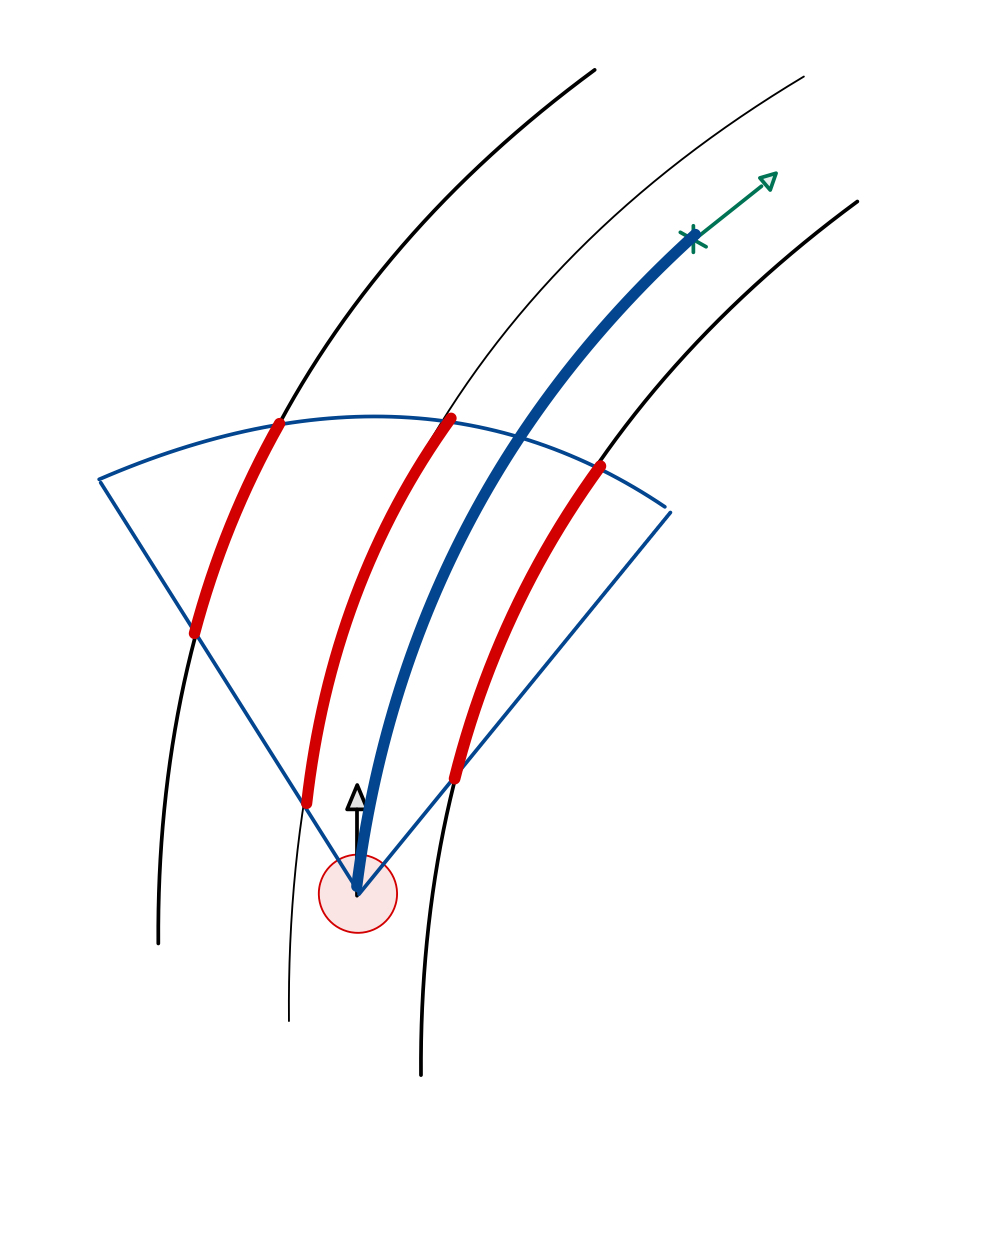
\includegraphics[width=\textwidth]{Pictures/lane following draw}
		\caption{lane following}
		\end{subfigure}	
	%\hskip2em
	\begin{subfigure}{.3\linewidth}
		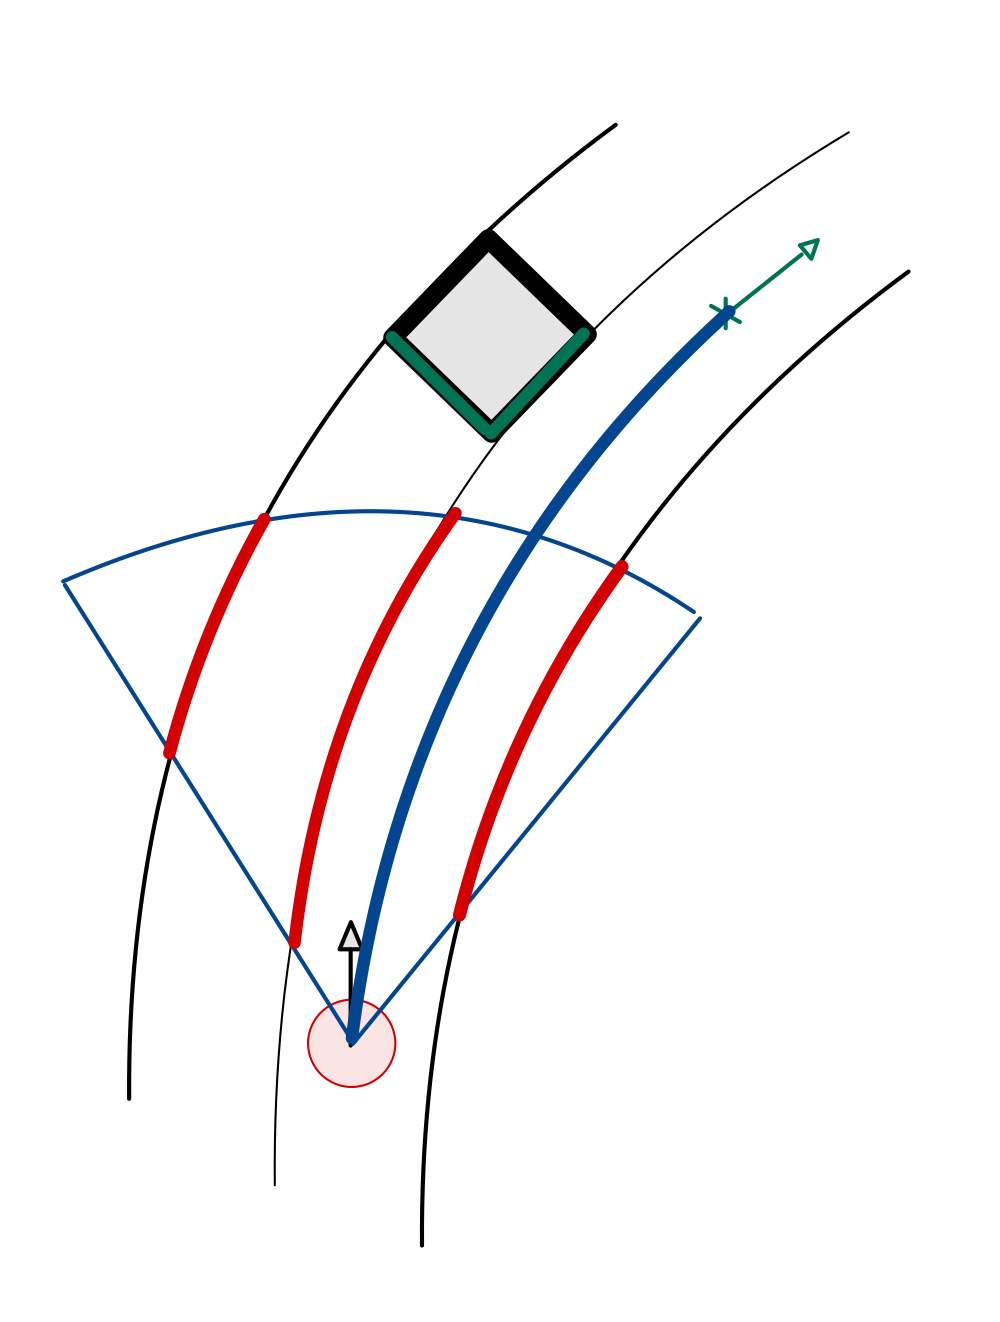
\includegraphics[width=\textwidth]{Pictures/passing obstacle}
		\caption{passing obstacle}
	\end{subfigure}
	%\hskip2em
	\begin{subfigure}{.3\linewidth}
		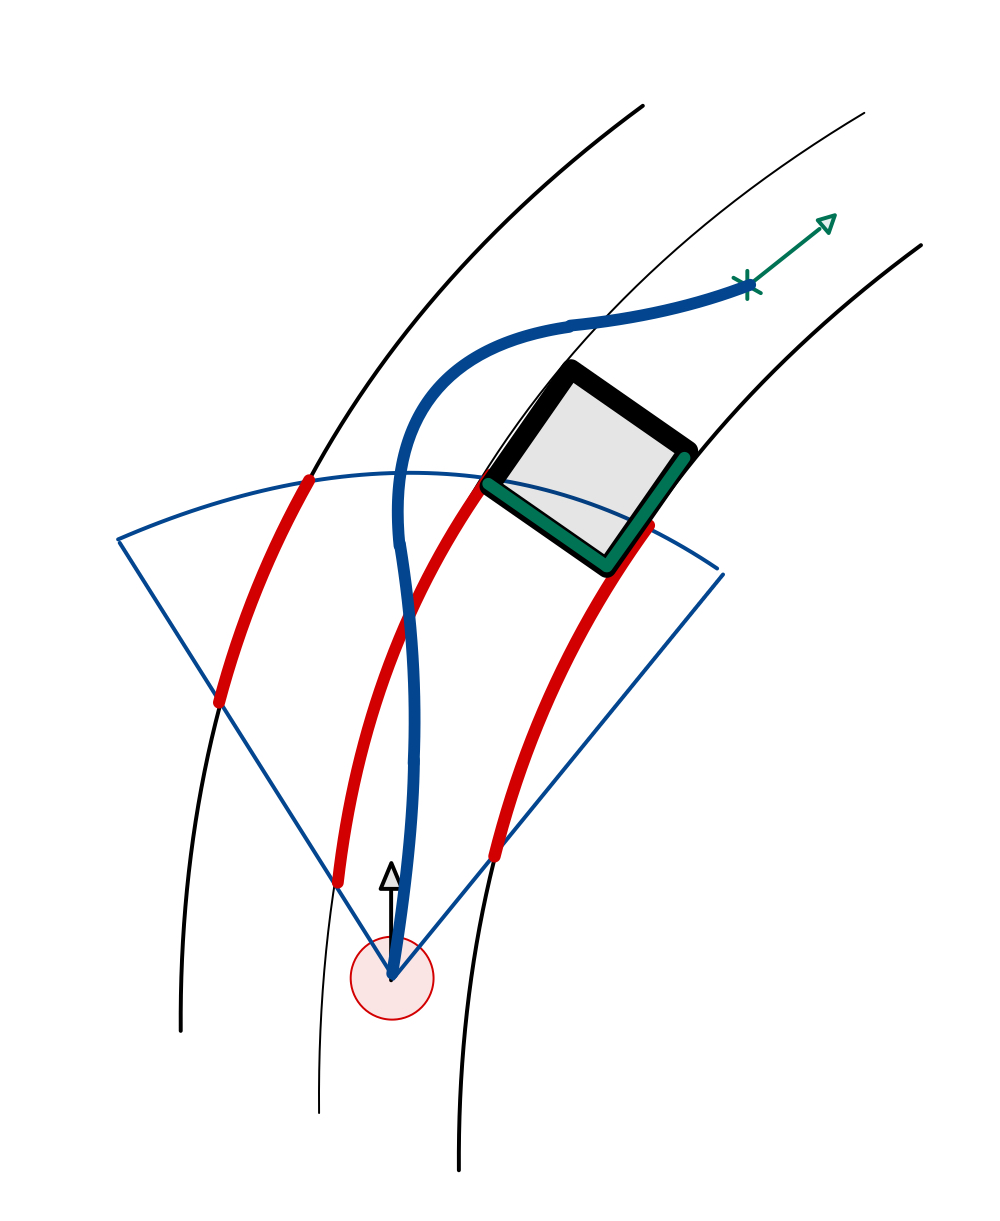
\includegraphics[width=\textwidth]{Pictures/obstaclee avoidance draw}
		\caption{obstacle avoidance}
	\end{subfigure}

	\caption{required driving behavior}
	\label{driving behavior}

\end{figure}

The wanted driving behavior is pictured in figure \ref{driving behavior}. The red arcs show the road markings, detected by the road detection. These can only be detected in the semi circle, since the road detection is restricted by the FOV (field of view) of the camera. In addition to that the road detection can only detect the road markings to a certain distance.

The green lines at the edge of the black square represent the obstacles detected by the lidar sensor.\\
Like described in the scope of this thesis the goal is, that the navigation avoids obstacles, if they block the right lane. Else the navigation is supposed to follow the right lane.

The robot navigates in a for itself totally unknown environment, while the navigation needs to be adaptable to the dynamics of the used and similar robots. Because the development of an entire stack, that would satisfies the previously mentioned requirements, exceeds the content of this thesis, an open source navigation project will be used which needs to cover the following points:
\begin{itemize}
	\item Goal pose input
	\item 2D mobile platform supporting conventional drive systems like ackermann and differential
	\item Path planning in respect to the robots kinematic and shape, as well as the environment detected by the sensors.
	\item Path planning and navigation in totally unknown environments
	\item Velocity output as linear and angular velocities
\end{itemize}










